% !TEX program = xelatex
\documentclass[a4paper,10pt]{article}

\usepackage[a4paper,top=1.5cm,bottom=1.55cm,left=1.55cm,right=1.55cm,headheight=13pt]{geometry}
\usepackage{fontspec}
\setmainfont{Times New Roman}
\setsansfont{Arial}
\usepackage{amsmath,amssymb,bm}
\usepackage{graphicx}
\usepackage{booktabs,array}
\usepackage{caption}
\usepackage{xcolor}
\usepackage{enumitem}
\usepackage{fancyhdr}
\usepackage{microtype}
\usepackage{titlesec}
\usepackage{flushend}
\usepackage{hyperref}

\definecolor{AcademicBlue}{HTML}{245A7A}
\definecolor{TextGray}{HTML}{4A5560}
\hypersetup{hidelinks,pdftitle={Teaching CLIP What Abnormal Means: A Mini-Paper on AA-CLIP},pdfauthor={Rpc}}
\graphicspath{{assets/paper-figures/}}
\setlength{\columnsep}{0.65cm}
\setlength{\emergencystretch}{1.5em}
\setlength{\parindent}{1em}
\setlength{\parskip}{0pt}
\linespread{0.97}
\setlist{nosep,leftmargin=1.5em}
\captionsetup{font=footnotesize,labelfont=bf,labelsep=quad,skip=4pt}
\titleformat{\section}{\large\bfseries}{\thesection}{0.75em}{}
\titleformat{\subsection}{\normalsize\bfseries}{\thesubsection}{0.65em}{}
\titlespacing*{\section}{0pt}{1.1ex plus 0.3ex minus 0.2ex}{0.45ex}
\titlespacing*{\subsection}{0pt}{0.9ex plus 0.2ex minus 0.2ex}{0.35ex}

\pagestyle{fancy}
\fancyhf{}
\fancyhead[L]{\small\color{TextGray}AA-CLIP Paper Paraphrase}
\fancyhead[R]{\small\color{TextGray}Rpc}
\fancyfoot[C]{\small\thepage}
\renewcommand{\headrulewidth}{0.35pt}

\newcommand{\TN}{T_{N}}
\newcommand{\TA}{T_{A}}
\newcommand{\loss}{\mathcal{L}}

\begin{document}
\fontsize{9.2pt}{10.5pt}\selectfont

\twocolumn[
\begin{@twocolumnfalse}
  \begin{center}
    {\Large\bfseries Teaching CLIP What ``Abnormal'' Means:\par}
    \vspace{0.15em}
    {\Large\bfseries A Mini-Paper on Anomaly-Aware CLIP\par}
    \vspace{0.45em}
    {\normalsize Rpc\par}
    {\small Paper Reading and Paraphrase Assignment, 11 August 2026\par}
  \end{center}

  \begin{abstract}
  Zero-shot anomaly detection aims to transfer knowledge from source categories to industrial products or medical images that were not observed during training. CLIP is an attractive backbone because of its broad image--text generalization, yet generic pre-training does not create a reliable direction that separates normal from abnormal states. This mini-paper paraphrases Anomaly-Aware CLIP (AA-CLIP), which first disentangles normal and anomalous semantics in the text space and then aligns multi-scale visual patch features with the resulting text anchors. The original CLIP parameters remain frozen; only shallow residual adapters and projection layers are optimized. Experiments on eleven industrial and medical benchmarks show strong image-level detection and pixel-level localization with limited source-domain data. The discussion also clarifies the scope of the zero-shot claim: AA-CLIP transfers to unseen target categories, but it is not training-free and still uses labeled source anomalies and pixel masks.
  \end{abstract}
  \noindent\textbf{Keywords:} zero-shot anomaly detection; CLIP; residual adapter; vision-language model; anomaly localization
  \vspace{0.55em}
\end{@twocolumnfalse}
]

\section{Introduction}

Anomaly detection identifies samples that depart from a normal distribution and, in segmentation settings, localizes the abnormal region. Conventional systems often require category-specific training data. This assumption is costly when defects or lesions are rare, diverse, and expensive to annotate. CLIP offers a transferable alternative because its contrastive image--text pre-training supports classification through textual descriptions such as ``a normal object'' and ``a damaged object'' \cite{radford2021}.

General semantic knowledge, however, is not equivalent to anomaly awareness. In the original CLIP space, normal and abnormal prompts for the same category can remain highly similar, and visibly defective images may be closer to a normal description. Ma et al. call this limitation \emph{anomaly unawareness} \cite{ma2025}. The central problem is therefore not merely to design a longer prompt, but to add a normal--abnormal decision direction without erasing CLIP's transferable category knowledge.

\section{Method}

\subsection{Controlled Residual Adaptation}

AA-CLIP freezes the CLIP backbone and inserts lightweight residual adapters after several shallow Transformer layers in both encoders. For a feature $x^i$ from layer $i$, the adapted representation is
\begin{align}
x_{\mathrm{res}}^i &= \operatorname{Norm}\!\left(\operatorname{Act}(W^i x^i)\right), \\
x_{\mathrm{enh}}^i &= \lambda x_{\mathrm{res}}^i+(1-\lambda)x^i .
\end{align}
The paper sets $\lambda=0.1$, so the original feature remains dominant while a small task-specific correction is introduced. This structure is intended to preserve zero-shot generalization better than unrestricted fine-tuning.

\subsection{Stage One: Text-Anchor Disentanglement}

The first stage freezes the image encoder and trains shallow text adapters and the final projector. Normal and abnormal prompts are encoded and averaged into anchors $\TN$ and $\TA$. Image-level binary cross-entropy and pixel-level Dice and Focal losses align these anchors with the training images:
\begin{equation}
\loss_{\mathrm{align}}
=\loss_{\mathrm{cls}}+\loss_{\mathrm{seg}}.
\end{equation}
A disentanglement term penalizes correlation between the anchors,
\begin{equation}
\loss_{\mathrm{dis}}=\left|\langle \TN,\TA\rangle\right|^2,
\end{equation}
and the total objective is $\loss_{\mathrm{total}}=\loss_{\mathrm{align}}+\gamma\loss_{\mathrm{dis}}$. The text encoder thus acquires an explicit normal--abnormal direction instead of relying on the original, entangled CLIP prompts.

\subsection{Stage Two: Patch-Feature Alignment}

The adapted text encoder is then fixed while residual adapters are trained on the image side. Features $F^i$ from layers 6, 12, 18, and 24 are projected into the text-feature dimension and aggregated:
\begin{equation}
V_{\mathrm{patch}}=\sum_{i=1}^{4}\operatorname{Proj}_{i}(F^i).
\end{equation}
Cosine similarities between $V_{\mathrm{patch}}$ and $[\TN,\TA]$ produce a pixel-level anomaly map; a global image feature produces the image-level prediction. The visual encoder therefore follows semantic anchors that have already been made anomaly-aware.

\begin{figure*}[t]
  \centering
  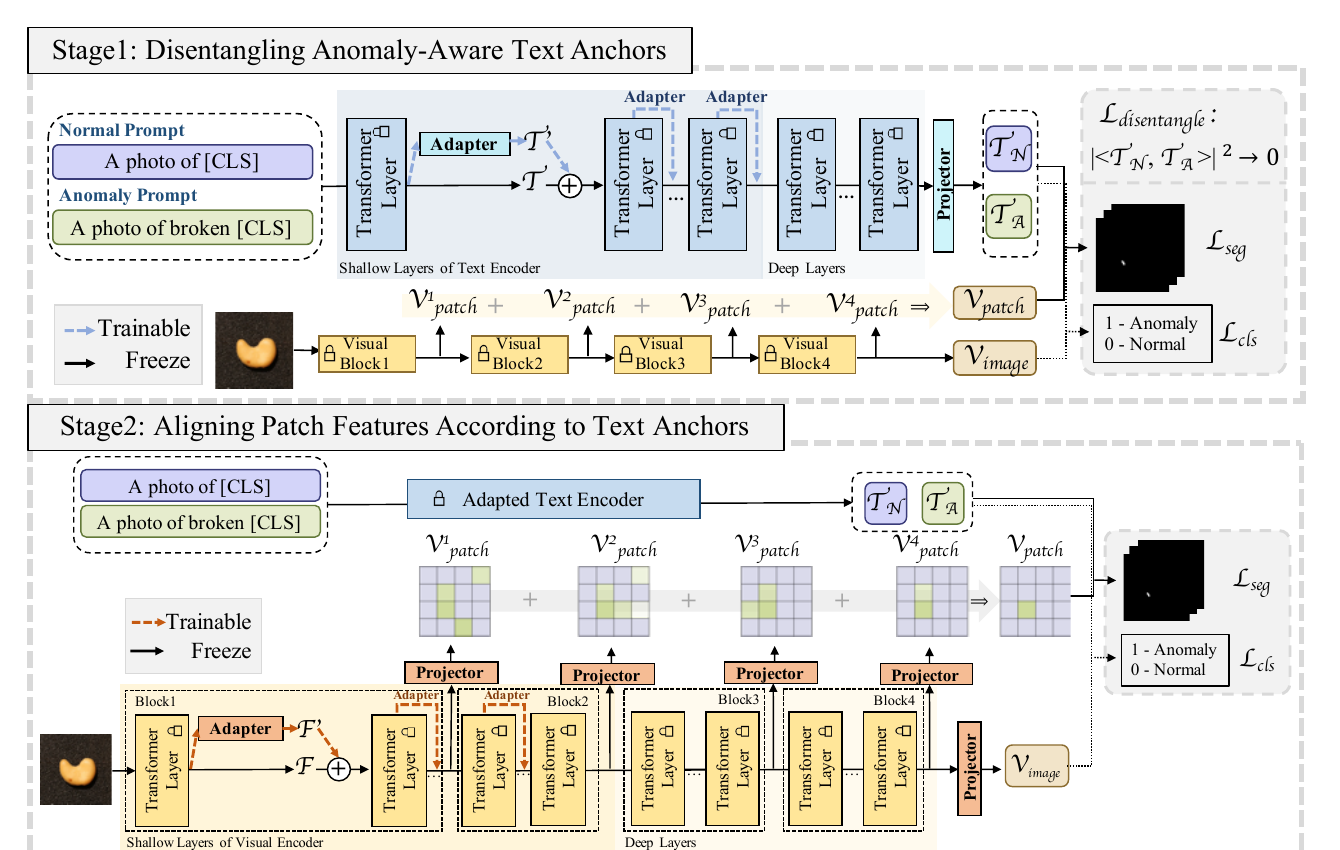
\includegraphics[width=0.82\textwidth]{fig4_pipeline.png}
  \caption{The two-stage AA-CLIP pipeline. Stage one constructs separable normal and anomaly anchors; stage two aligns multi-scale patch features with the fixed anchors. Cropped from Fig.~4 of the source paper under CC BY 4.0.}
  \label{fig:pipeline}
  \vspace{0.45em}

  \begin{minipage}[t]{0.46\textwidth}
    \centering\footnotesize
    \captionof{table}{Average AUROC (\%) at different training scales \cite{ma2025}}
    \label{tab:shots}
    \begin{tabular}{lcc}
      \toprule
      Training scale & Pixel & Image \\
      \midrule
      2-shot  & 92.0 & 78.1 \\
      16-shot & 92.6 & 81.8 \\
      64-shot & 92.8 & \textbf{83.1} \\
      Full    & \textbf{93.4} & 82.5 \\
      \bottomrule
    \end{tabular}
  \end{minipage}
  \hfill
  \begin{minipage}[t]{0.46\textwidth}
    \centering\footnotesize
    \captionof{table}{Core ablation results (AUROC, \%) \cite{ma2025}}
    \label{tab:ablation}
    \begin{tabular}{lcc}
      \toprule
      Configuration & Pixel & Image \\
      \midrule
      Visual residual adapter & 91.3 & 80.7 \\
      $+$ Text residual adapter & 92.1 & 82.6 \\
      $+$ Disentanglement loss & \textbf{92.7} & \textbf{83.3} \\
      \bottomrule
    \end{tabular}
  \end{minipage}
\end{figure*}

\section{Experiments and Results}

\subsection{Evaluation Protocol}

The evaluation covers four industrial datasets---MVTec AD, VisA, BTAD, and MPDD---and seven medical datasets spanning brain MRI, liver CT, retinal OCT, and colon polyp images. Training uses 2, 16, or 64 samples per class, or the full source dataset, while testing is performed on different datasets and unseen categories. The backbone is OpenCLIP ViT-L/14 with $518\times518$ inputs. Image-level and pixel-level AUROC measure detection and localization performance.

The 2-shot setting still contains both normal and anomalous examples, and training uses image labels and pixel masks. ``Zero-shot'' therefore refers to unseen target categories rather than an absence of anomaly supervision.

\subsection{Main Results}

Table~\ref{tab:shots} summarizes the average results. Pixel-level AUROC reaches 93.4\% with full training data, while image-level AUROC peaks at 83.1\% with 64 samples per class. The 2-shot pixel-level score is already 92.0\%, indicating efficient adaptation. The image-level decline from 83.1\% at 64-shot to 82.5\% with full data is consistent with adaptation saturation or overfitting.

\subsection{Ablation Evidence}

The VisA-trained 64-shot ablation in Table~\ref{tab:ablation} explains the mechanism. An ordinary adapter reduces pixel- and image-level AUROC to 48.9\% and 53.4\%, showing that aggressive feature modification can destroy generalization. A visual residual adapter recovers 91.3\% and 80.7\%. Text adaptation and the disentanglement loss further raise the final scores to 92.7\% and 83.3\%. The gain therefore depends on both controlled visual adaptation and a more separable text space.

\section{Critical Discussion}

AA-CLIP's main contribution is not a larger backbone but a better geometry for the target decision. Adapting text before vision separates the task of defining abnormality from the task of localizing its evidence. Frozen backbones, residual mixing, and staged training jointly reduce catastrophic forgetting. The reported feature-space separation and the cross-dataset metrics provide complementary evidence that the change is not limited to the training categories.

Three limitations remain. First, the method relies on labeled source anomalies and pixel masks, so it should not be described as unsupervised anomaly detection. Second, full-data training does not continue to improve average image-level performance, which makes hyper-parameter control important. Third, the paper emphasizes AUROC rather than cross-domain calibration, latency, or confidence reliability. Future work could study weakly supervised text anchors, broader anomaly diversity, deployment calibration, and explicit modelling of false-positive and false-negative costs in medical settings.

For the visual research direction I am considering, the more important question is not how many adaptation modules can be added, but whether the benefit of a semantic anchor and a controlled visual residual survives shifts in products, illumination, and imaging conditions. My working hypothesis is that stabilizing text semantics first and then searching for local evidence through a bounded residual is more likely to preserve cross-domain generalization than directly fine-tuning the whole foundation model. I would therefore evaluate calibration error, memory use, latency, and failure cases together with AUROC, so that a higher benchmark score is not confused with greater reliability in deployment.

\section{Conclusion}

AA-CLIP can be summarized in one sentence: first teach the text space what abnormality means, then make visual patches search for that meaning. Its two-stage residual adaptation adds an anomaly-specific direction without broadly rewriting CLIP, yielding competitive cross-category performance with limited source data. Prompt engineering alone is insufficient when the embedding space lacks the distinction required by the task.

\begin{thebibliography}{9}
\small
\bibitem{ma2025}
W. Ma, X. Zhang, Q. Yao, et al., ``AA-CLIP: Enhancing zero-shot anomaly detection via anomaly-aware CLIP,'' in \emph{Proceedings of the IEEE/CVF Conference on Computer Vision and Pattern Recognition}, 2025.

\bibitem{radford2021}
A. Radford, J. W. Kim, C. Hallacy, et al., ``Learning transferable visual models from natural language supervision,'' in \emph{Proceedings of the 38th International Conference on Machine Learning}, pp. 8748--8763, 2021.

\bibitem{jeong2023}
J. Jeong, Y. Zou, T. Kim, et al., ``WinCLIP: Zero-/few-shot anomaly classification and segmentation,'' in \emph{Proceedings of the IEEE/CVF Conference on Computer Vision and Pattern Recognition}, pp. 19606--19616, 2023.
\end{thebibliography}

\end{document}
